\documentclass[12pt, aspectratio=43]{beamer} 

% 自訂字體的封包
\usepackage{fontspec} 

%% 設定中文字體
\usepackage{xeCJK}
    \setCJKmainfont[AutoFakeBold=3]{SimSun}
    \XeTeXlinebreaklocale "zh"             
    \XeTeXlinebreakskip = 0pt plus 1pt

% 數學工具及符號
\usepackage{mathtools, amsmath, amsfonts, amsthm, amssymb, latexsym} 
\usepackage{relsize}
% background
\usetheme{Darmstadt}
\setbeamertemplate{footline}[page number]{}

% Headers and footers
\usepackage{fancyhdr}

% Inserting Images
\usepackage{graphicx}
\usepackage{subcaption}
\usepackage{float}


% Using colours in LaTeX
\usepackage{color}
\usepackage{multirow}

% Biblatex citation styles
\usepackage[style=numeric,backend=bibtex,sorting=none]{biblatex} 
\bibliography{reference}

% Misc
\usepackage{lipsum}
\usepackage{wrapfig}
\usepackage[document]{ragged2e}
\usepackage{tabularx}
\usepackage{tikz}

\usepackage{hyperref}

\setbeamertemplate{caption}[numbered]
 % 載入封包與文檔配置

% Title, Subtitle, Author, Institute, Date
\title[\textbf{Week 5 Report}]{Week 5 Report}
\author[Chen, Pin-Jui]{Chen, Pin-Jui}
\date[Oct 17, 2025]{Oct 17, 2025}

\begin{document}

% Title page frame
\begin{frame}
  \titlepage
\end{frame}

% Index
\begin{frame}
  \frametitle{Index}
  \tableofcontents
\end{frame}

\section{RSEM: accurate transcript quantification from RNA-Seq data with or without a reference genome}

\begin{frame}{Read}
	\begin{figure}[h!]
		\centering
		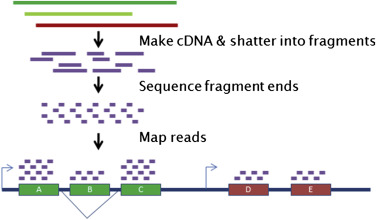
\includegraphics[width=0.8\linewidth]{Figure/Read.jpg}
	\end{figure}
\end{frame}

\begin{frame}{Alternative Splicing}
	\begin{figure}[h!]
		\centering
		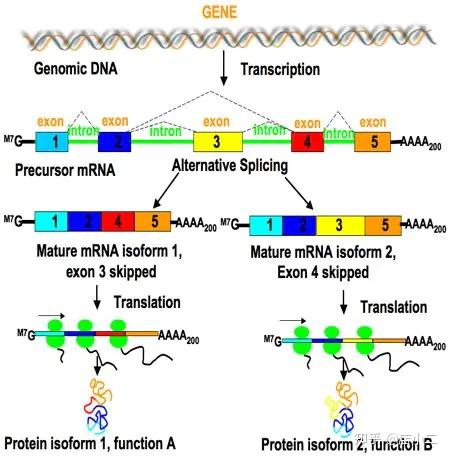
\includegraphics[width=0.6\linewidth]{Figure/splicing.jpg}
	\end{figure}
\end{frame}

\begin{frame}{count}
	\begin{figure}[h!]
		\centering
		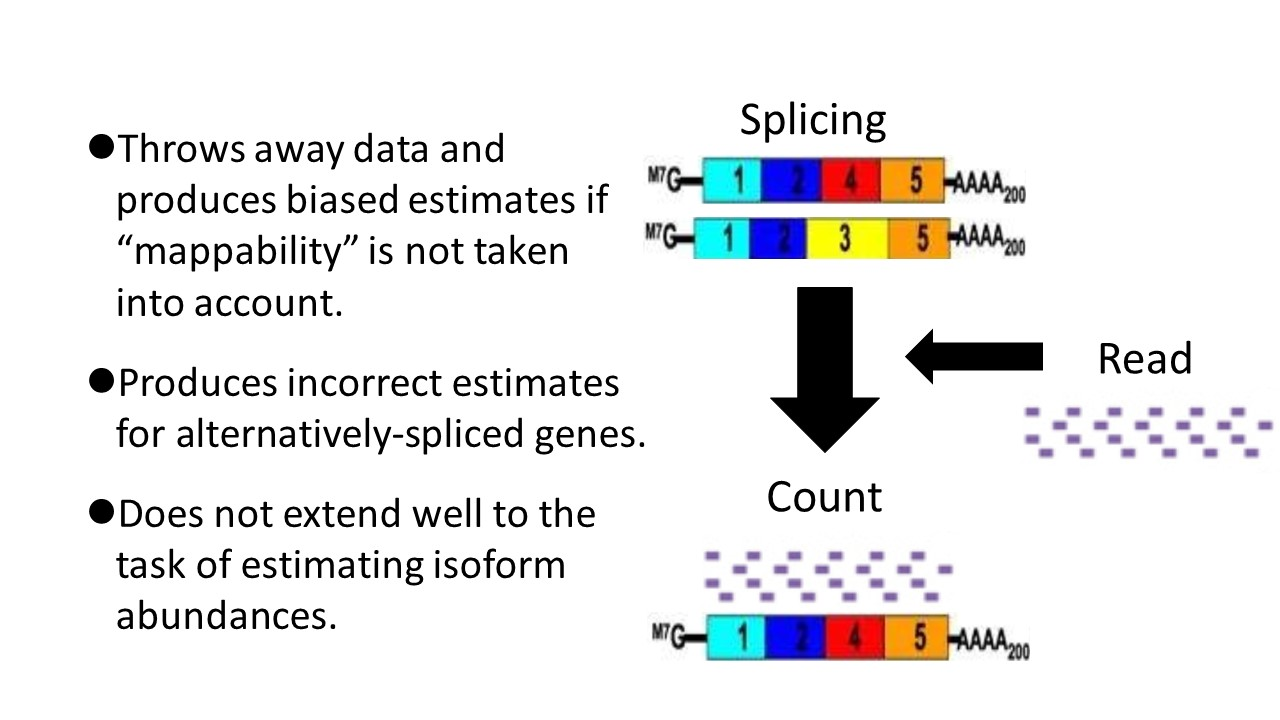
\includegraphics[width=\linewidth]{Figure/old_count.jpg}
	\end{figure}
\end{frame}

\begin{frame}{RSEM}
	\begin{figure}[h!]
		\centering
		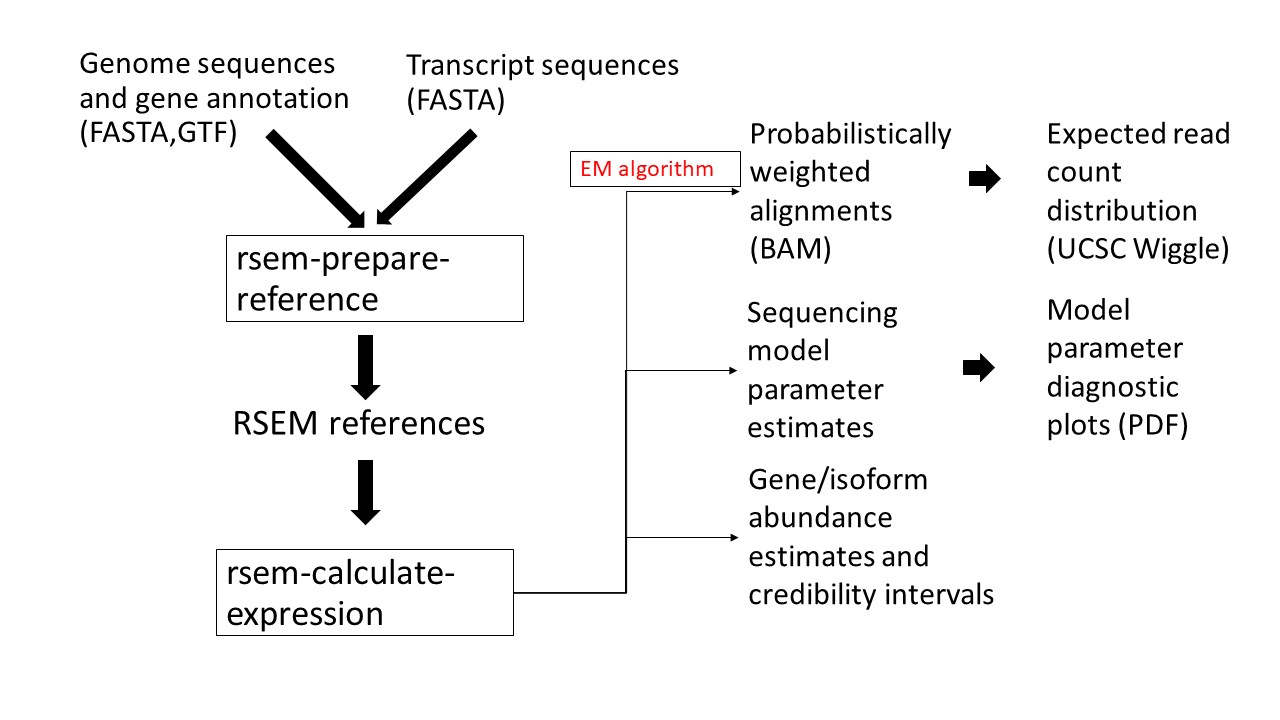
\includegraphics[width=1.1\linewidth]{Figure/RSEM.jpg}
	\end{figure}
\end{frame}


\begin{frame}[allowframebreaks]{參考文獻}
    \printbibliography % 使用 biblatex 的指令來列印參考文獻
\end{frame}



\end{document}
